\documentclass[10pt,a4paper,UTF8]{ctexart}
\usepackage{geometry}%用于设置上下左右页边距
	\geometry{left=2.5cm,right=2.5cm,top=3.2cm,bottom=2.8cm}
\usepackage{xeCJK,amsmath,paralist,enumerate,booktabs,multirow,graphicx,subfig,setspace,listings,lastpage,hyperref}
\usepackage{amsthm, amssymb, bm, color, framed, graphicx, hyperref, mathrsfs}
\usepackage{mathrsfs}  
	\setlength{\parindent}{2em}
	\lstset{language=Matlab}%
\usepackage{fancyhdr}
\usepackage{graphicx}
\usepackage{listings}
\usepackage{xcolor}
\usepackage{float}

\definecolor{mKeyword}{RGB}{0,0,255}          % bule
\definecolor{mString}{RGB}{160,32,240}        % purple
\definecolor{mComment}{RGB}{34,139,34}        % green
\definecolor{mNumber}{RGB}{128,128,128} 

\lstdefinestyle {njulisting} {
	basewidth = 0.5 em,
	lineskip = 3 pt,
	basicstyle = \small\ttfamily,
	% keywordstyle = \bfseries,
	commentstyle = \itshape\color{gray}, 
	basicstyle=\small\ttfamily,
	keywordstyle={\color{mKeyword}},     % sets color for keywords
	stringstyle={\color{mString}},       % sets color for strings
	commentstyle={\color{mComment}},     % sets color for comments
	numberstyle=\tiny\color{mNumber},
	numbers = left,
	captionpos = t,
	breaklines = true,
	xleftmargin = 2 em,
	xrightmargin = 2 em,
	frame=tlrb
}

\lstset{
style = njulisting, % 调用上述样式 
flexiblecolumns % 允许调整字符宽度
}

\pagestyle{fancy}
\lhead{\textsc{Foundation of Computing System}}
\rhead{\textsc{Nanjing University}}
\cfoot{\thepage}
\renewcommand{\headrulewidth}{0.4pt}
\renewcommand{\theenumi}{(\arabic{enumi})}


\definecolor{shadecolor}{RGB}{241, 241, 255}

\newcommand{\problemname}{待定义}
\newenvironment{problem}{\begin{shaded}\par\noindent\textbf{题目\  \problemname}}{\end{shaded}\par}
\newenvironment{solution}{\par\noindent\textbf{解答}\ }{\par}
\newenvironment{note}{\par\noindent\textbf{题目 \problemname 的注记}}{\par}

\begin{document}

\begin{center}
\LARGE\textbf{第八章习题参考答案}
\end{center}

{\kaishu 包含题目:习题$8.2-8.4$}




\renewcommand{\problemname}{8.2}
\begin{problem}
	下表显示了一个小的存储器的部分情况,根据此表回答以下问题。
	\begin{enumerate}[(1)]
		\item 单元0和单元4包含的二进制数值分别是什么?
		\item 每个单元内的二进制数值可以以不同的方式解释,如可以表示为无符号整数、
		补码整数、浮点数、ASCII码等
			\begin{enumerate}[I.]
				\item 将单元0和单元1解释为8位补码整数,并以十进制形式写出结果。
				\item 将单元2和单元3解释为8位无符号整数,并以十进制形式写出结果。
				\item 将单元4解释为ASCII码值。
				\item 将单元4、5、6和7解释为一个IEEE浮点数(32位),其中单元4包含该数的[31:24]位,
				单元5包含[23:16]位,单元6包含[15:8]位,单元7包含[7:0]位,以十进制形式写出结果
			\end{enumerate}
		\item 存储单元的内容也可以是一条指令,将单元8、9、10和11解释为一条指令,其中单元8包含该指令的
		[31:24]位,单元9包含[23:16]位,单元10包含[15:8]位,单元11包含[7:0]位,该指令表示什么?
		\item 一个二进制数值也可以被解释为一个存储单元的地址,如果存储在单元11中的数值是一个地址,
		它指的是哪个单元?该单元里包含的二进制数值是什么?
	\end{enumerate}
\end{problem}

\begin{figure}[H]
	\centering
	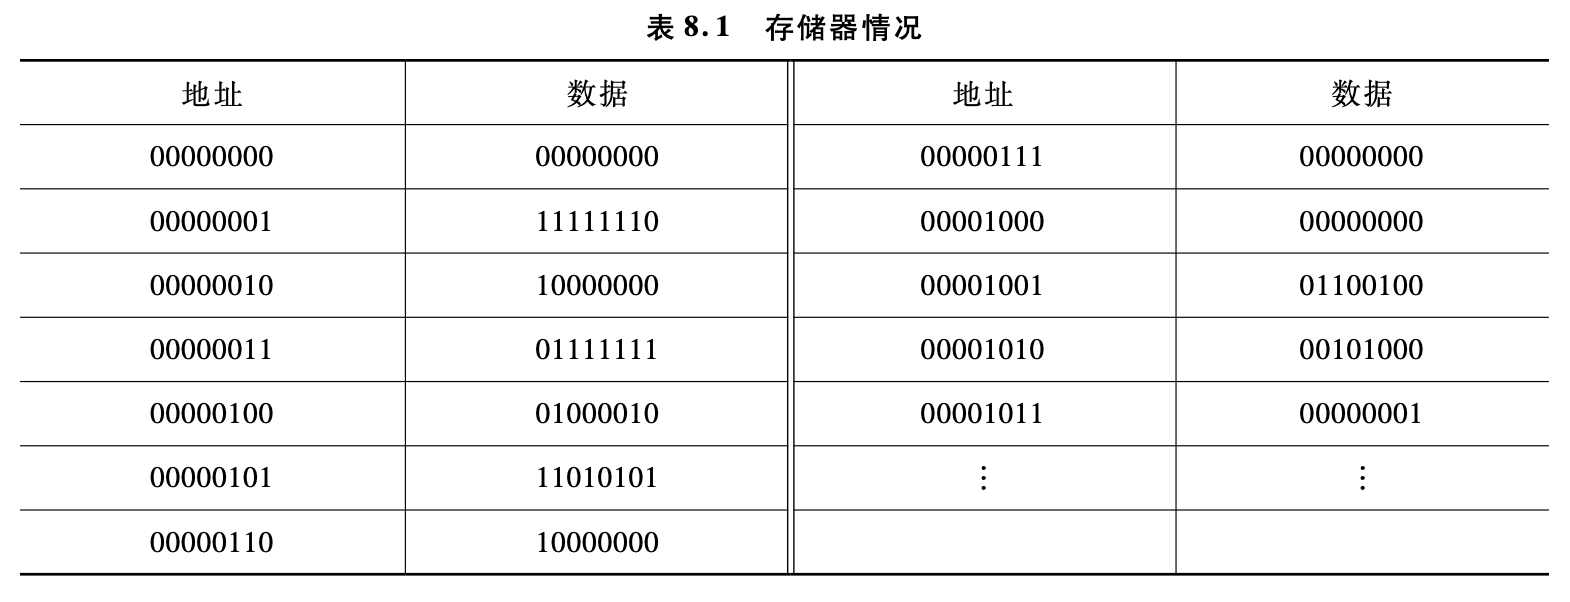
\includegraphics[scale=0.5]{img/8.2.png}
\end{figure}

\begin{solution}
	\begin{enumerate}[(1)]
		\item 0;66
		\item \begin{enumerate}[I.]
			\item 0;$-2$
			\item 128;127
			\item B
			\item 0 10000101 10101011000000000000000 = 106.75
		\end{enumerate}
		\item 将R3和R4中的数相加,结果存到R5中
		\item 单元11中存储的是00000001,即单元1;那个单元中的二进制数值为11111110,即$-2$
	\end{enumerate}

\end{solution}


\renewcommand{\problemname}{8.3}
\begin{problem}
	假设一个16位的指令采取如下图所示格式,如果共有12个操作码和8个寄存器,
	那么“补码整数”能够表示的数值范围是什么?
\end{problem}

\begin{figure}[H]
	\centering
	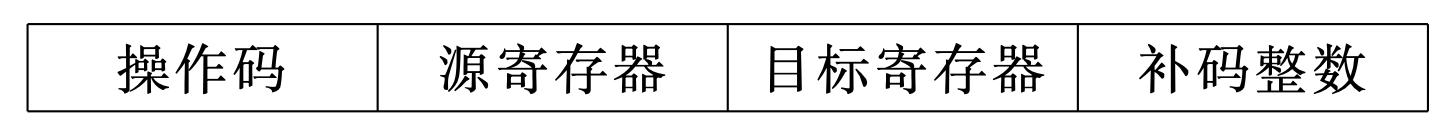
\includegraphics[scale=0.3]{img/8.3.png}
\end{figure}

\begin{solution}
	$-2^5\sim 2^5-1$,即$-32\sim 31$
\end{solution}


\renewcommand{\problemname}{8.4}
\begin{problem}
	假设一个32位的指令采取如下图所示格式,如果共有200个操作码和60个寄存器,
	“无符号整数”能够表示的最大数是多少?
\end{problem}

\begin{figure}[H]
	\centering
	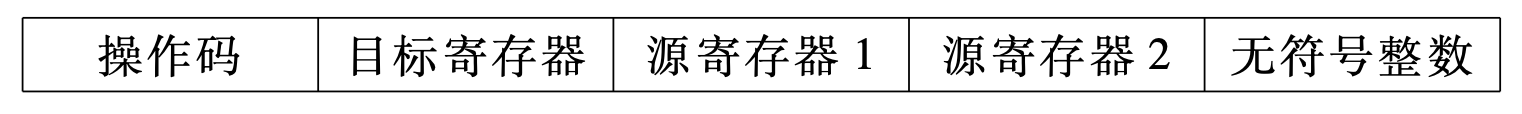
\includegraphics[scale=0.35]{img/8.4.png}
\end{figure}

\begin{solution}
	$2^6-1=63$
\end{solution}


\end{document}
